\documentclass{article}
\usepackage[utf8]{inputenc}
\usepackage[T1]{fontenc}
\usepackage[french]{babel}
\usepackage{graphicx}

\title{Rendu n.1 Projet technologique}
\author{Zoé Debaty}
\date{November 2019}

\begin{document}

\maketitle
\tableofcontents 
\newpage

% --------- Specificites techniques --------- %
\section{Spécificités techniques}

% --- L'image --- %
\subsection{L'image}
\begin{center} 
    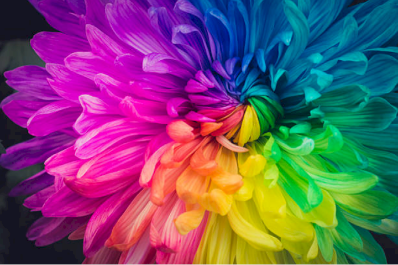
\includegraphics[width=9cm]{../multicolor}
    
    Image de base.
\end{center}
\bigbreak

\begin{itemize}
\item Nom : "multicolor"
\item Dimensions : 612p * 408p
\item Taille : 59,9 Ko
\end{itemize}
\medbreak

L'image a été choisie car elle possède des changements de luminosité et énormément de couleurs afin de tester au mieux mes fonctions.
C'est la seule image sur laquelle mon application a été testée pour l'instant.

% --- Le telephone --- %
\subsection{Le téléphone}
Pour tester mes fonctions j'utilise un Sony Xperia XA, avec un écran de 5 pouces.
Il tourne sous Android Nougat 7.0.
\medbreak

J'ai aussi pu tester avec un Neffos X1 avec un écran de 5 pouces.
Il tourne lui aussi sous Android Nougat 7.0.
\newpage

% ---------------- Fonctions ---------------- %
\section{Fonctions}

\subsection{Fonctions de TD}

% --- Version grise --- %
\subsubsection{Version grise \underline{TD 1 Question 3}}
Cette fonction grise l'image.
\bigbreak

\begin{center} 
    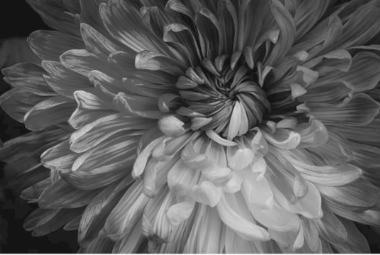
\includegraphics[width=9cm]{../Image_fonctions/Gris}

    Image de base grisée
\end{center}
\bigbreak

\begin{center} 
    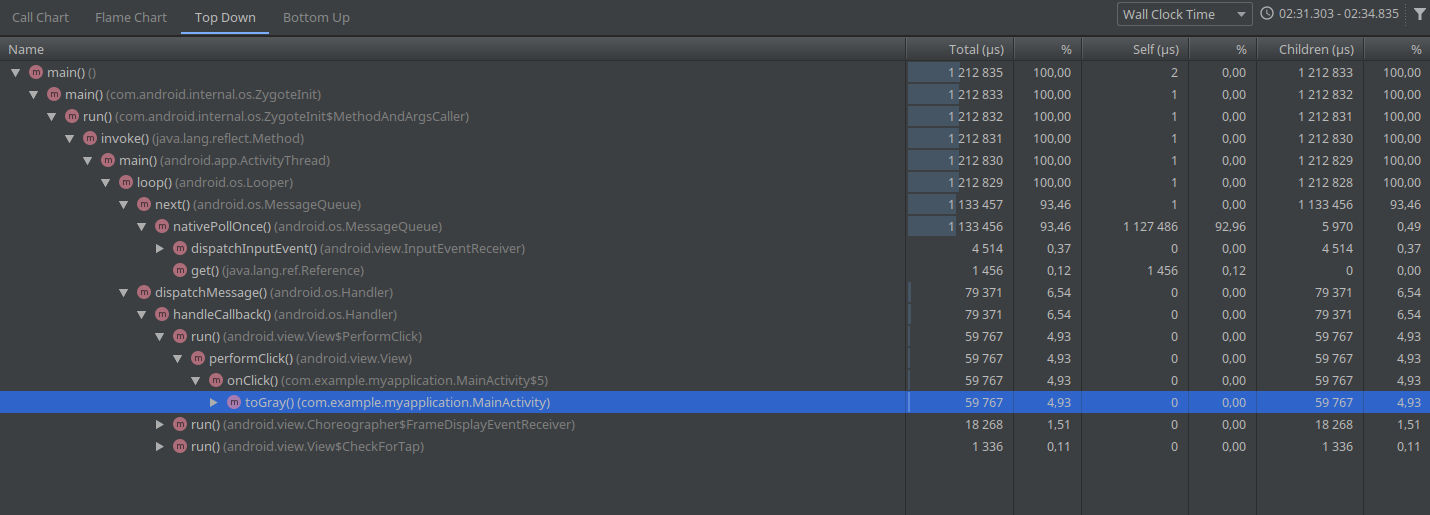
\includegraphics[width=11cm]{../Image_temps/TempsToGray}

    Temps de traitement de la fonction ToGray()
\end{center}
\bigbreak

% --- Couleur aleatoire --- %
\subsubsection{Couleur aléatoire \underline{TD 2 Question 2.1}}
Cette fonction permet de coloriser l'image avec une couleur choisie aléatoirement.
\bigbreak

\begin{center} 
    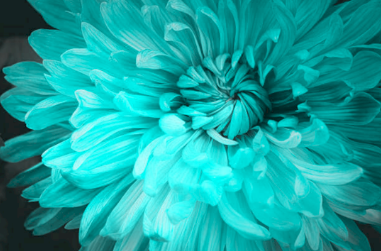
\includegraphics[width=9cm]{../Image_fonctions/RandomCouleur1}

    Image colorisée avec une couleur aléatoire (exemple 1)
\end{center}
\bigbreak

\begin{center} 
    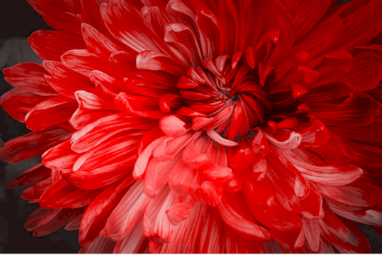
\includegraphics[width=9cm]{../Image_fonctions/RandomCouleur2}

    Image colorisée avec une couleur aléatoire (exemple 2)
\end{center}
\bigbreak

\begin{center} 
    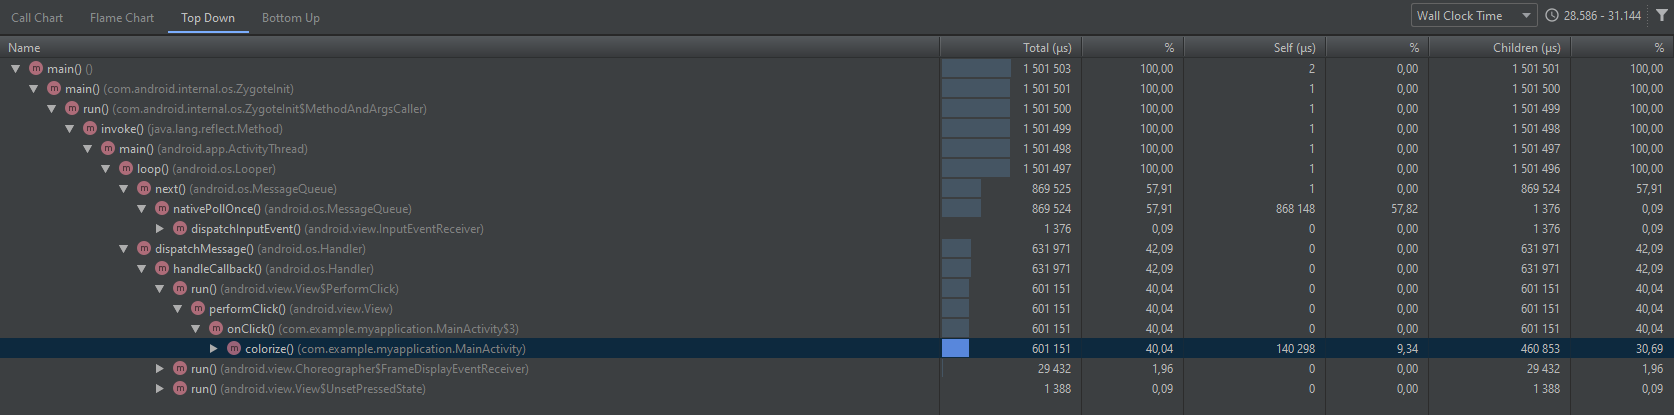
\includegraphics[width=11cm]{../Image_temps/TempsColorize}

    Temps de traitement de la fonction colorize()
\end{center}
\bigbreak

% --- Selection de couleurs --- %
\subsubsection{Selection de couleurs \underline{TD 2 Question 2.2}}
Cette fonction permet, au moyen de deux limites (qu'on modifie de 10 en 10), d'afficher ou non certaines couleurs.
\bigbreak

\begin{center} 
    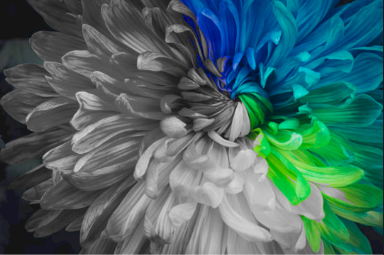
\includegraphics[width=9cm]{../Image_fonctions/SelectedColor}

    Image de base avec les deux limites n'affichants que les parties bleus et vertes de l'image.
\end{center}
\bigbreak

\begin{center} 
    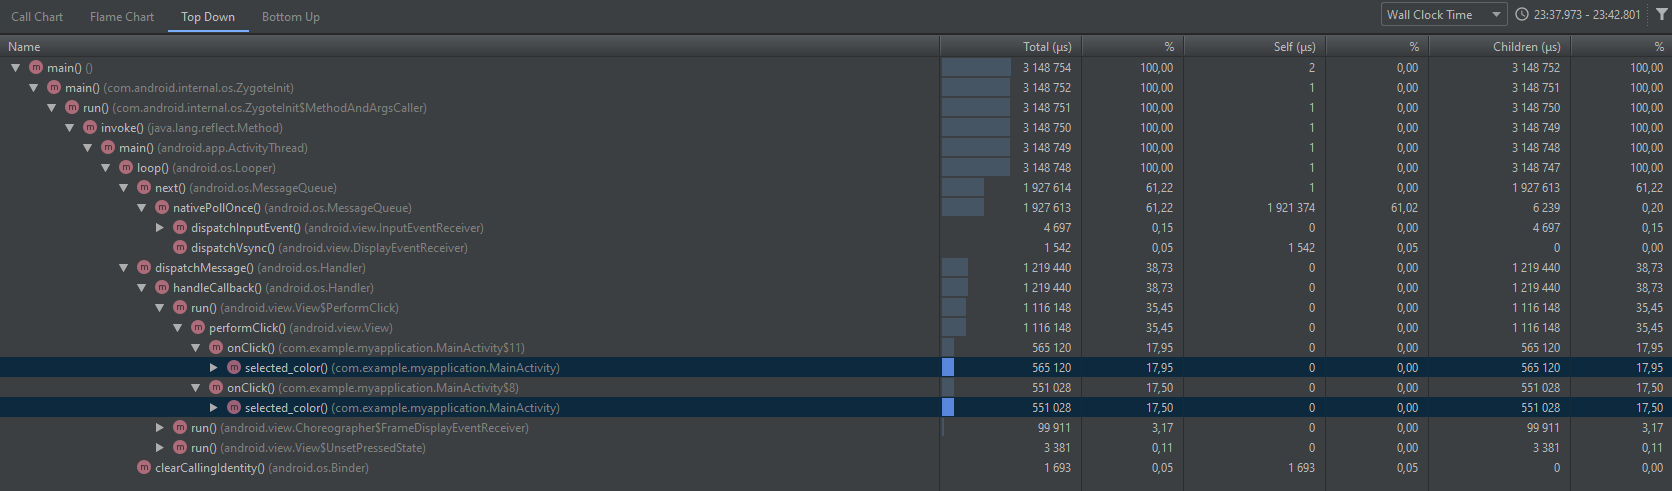
\includegraphics[width=11cm]{../Image_temps/TempsSelectedColor}

    Temps de traitement de la fonction selected\_color() appelée deux fois\\(+10 gauche et -10 droit).
\end{center}
\bigbreak

% --- Extension lineaire --- %
\subsubsection{Extension linéaire \underline{TD 3 Question 1.1}}
Cette fonction est l'implémentation de l'augmentation du contraste par extension de dynamique.
\bigbreak

\begin{center} 
    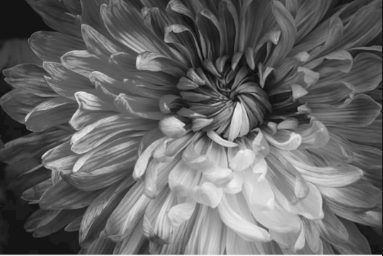
\includegraphics[width=9cm]{../Image_fonctions/ExtensionLineaire}

    Image de base grisée puis modifiée avec l'extension linéaire.
\end{center}
\bigbreak

\begin{center} 
    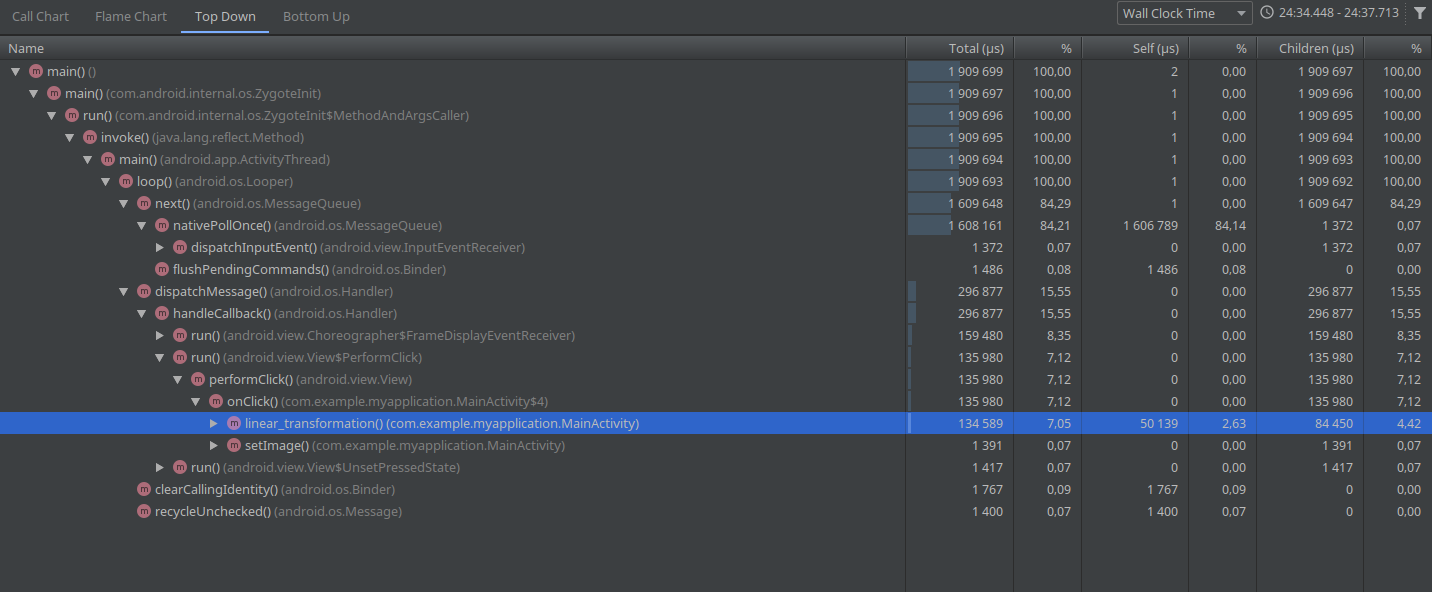
\includegraphics[width=11cm]{../Image_temps/TempsLinearTransformation}

    Temps de traitement de la fonction linear\_transformation()
\end{center}
\bigbreak

\subsection{Autres fonctions}

% --- Reinitialisation --- %
\subsubsection{Réinitialisation}
Cette fonction permet de remettre l'image de base en image constante et donc d'annuler toutes les modifications effectuée auparavant.
\bigbreak

\begin{center} 
    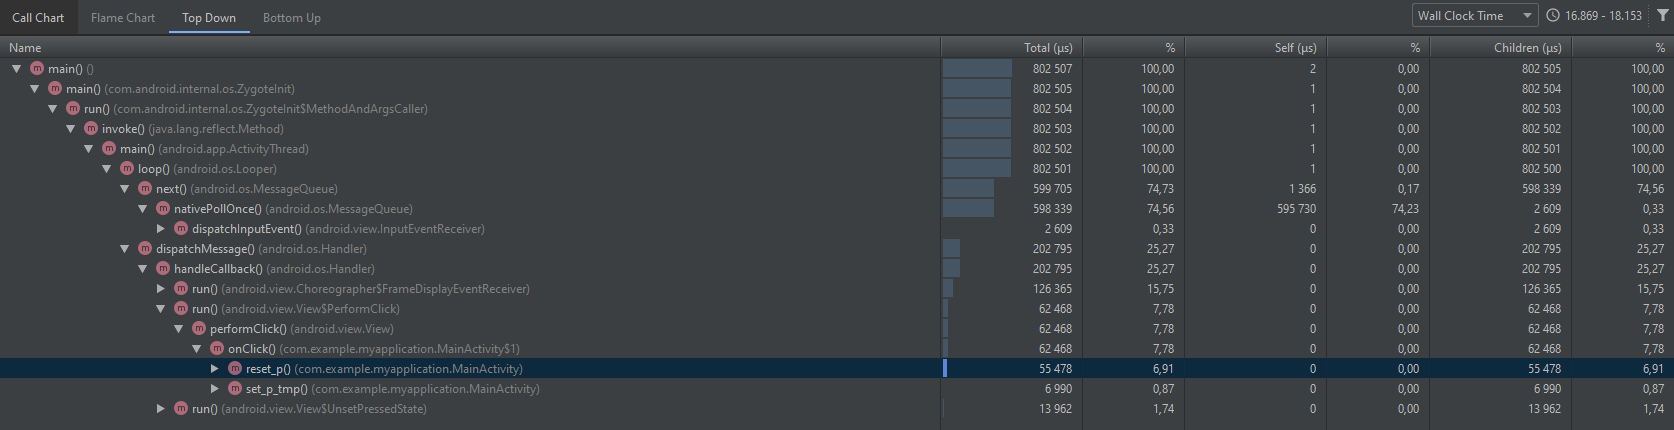
\includegraphics[width=11cm]{../Image_temps/TempsReset}

    Temps de traitement de la fonction reset() sur l'image de base passée en négatif.
\end{center}
\bigbreak

% --- Saturation --- %
\subsubsection{Saturation}
Cette fonction permet de modifier la saturation de l'image HSV par tranche de +- 10 \%.
\bigbreak

\begin{center} 
    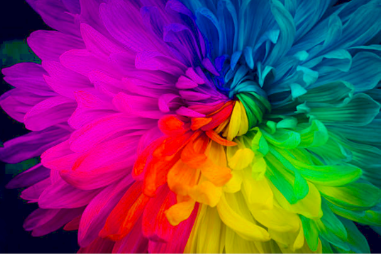
\includegraphics[width=9cm]{../Image_fonctions/SaturationMax}

    Image de base avec la saturation au maximum.
\end{center}
\bigbreak

\begin{center} 
    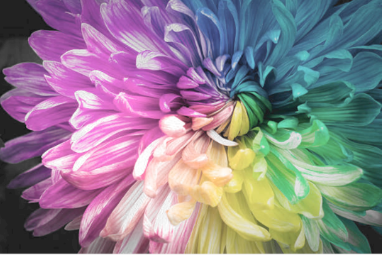
\includegraphics[width=9cm]{../Image_fonctions/SaturationMoins6}

    Image de base avec 60\% de saturation en moins.
\end{center}
\bigbreak

\begin{center} 
    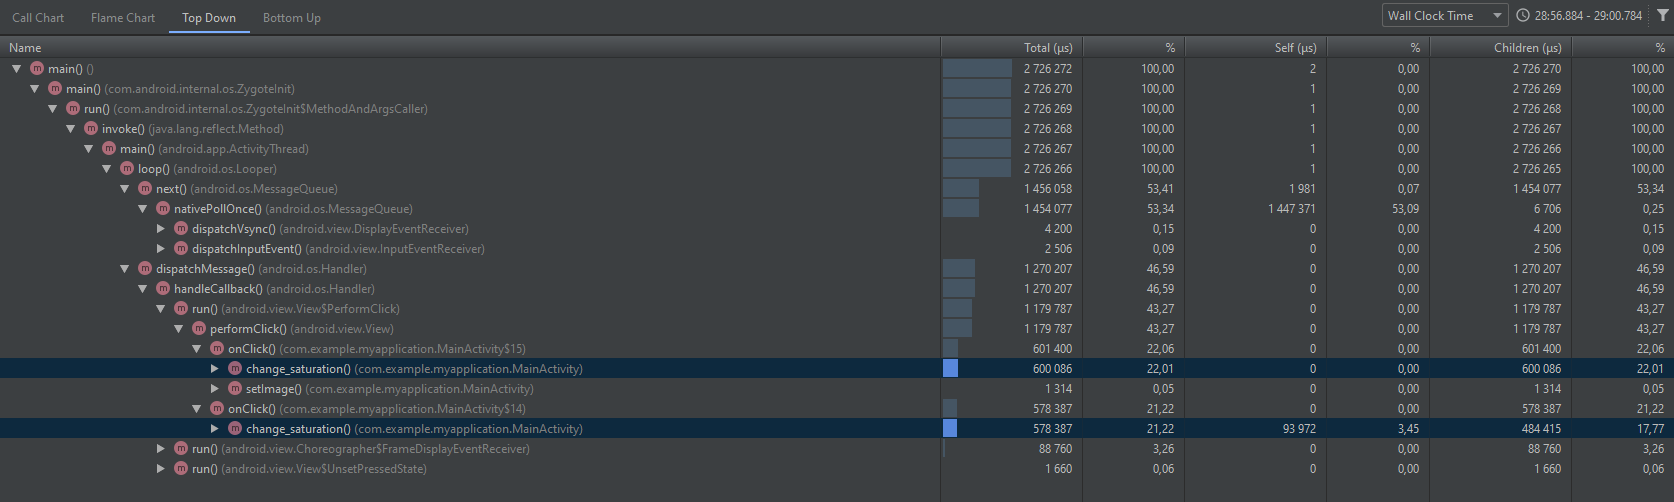
\includegraphics[width=11cm]{../Image_temps/TempsChangeSaturation}

    Temps de traitement de la fonction change\_saturation() appelé deux fois (+1 et -1).
\end{center}
\bigbreak

% --- Luminosite --- %
\subsubsection{Luminosité}
Cette fonction permet de changer la luminosité de l'image HSV par tranche de +- 10 \%.
\bigbreak

\begin{center} 
    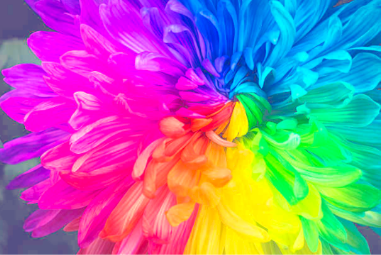
\includegraphics[width=9cm]{../Image_fonctions/LuminositePlus3}

    Image de base avec 30\% de luminosité en plus.
\end{center}
\bigbreak

\begin{center} 
    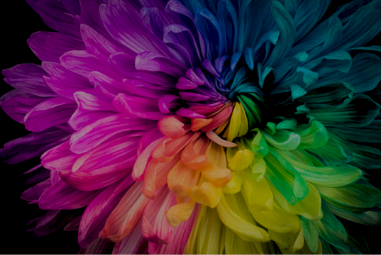
\includegraphics[width=9cm]{../Image_fonctions/LuminositeMoins3}

    Image de base avec 30\% de luminosité en moins.
\end{center}
\bigbreak

\begin{center} 
    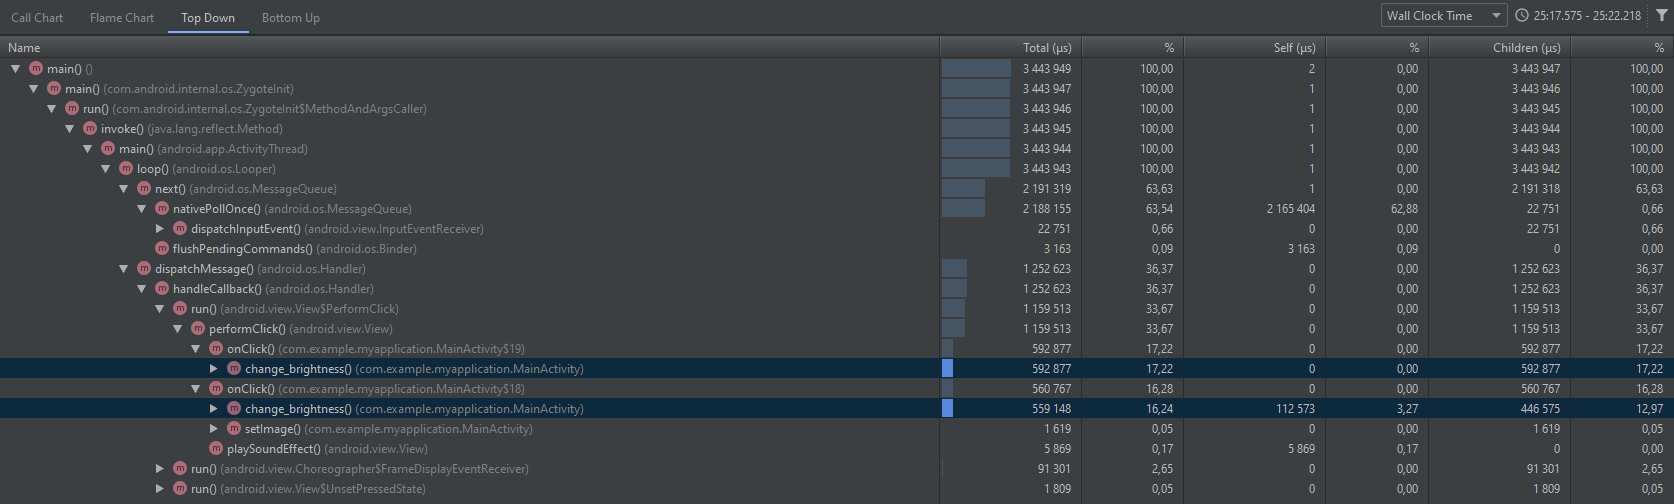
\includegraphics[width=11cm]{../Image_temps/TempsChangeBrightness}

    Temps de traitement de la fonction change\_brightness() appelée deux fois\\(+1 et -1).
\end{center}
\bigbreak

% --- Negatif --- %
\subsubsection{Négatif}
Cette fonction passe l'image en négatif.
\bigbreak

\begin{center} 
    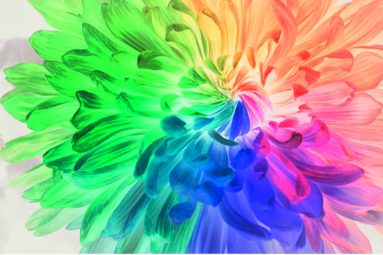
\includegraphics[width=9cm]{../Image_fonctions/Negatif}

    Image de base en négatif
\end{center}

\begin{center} 
    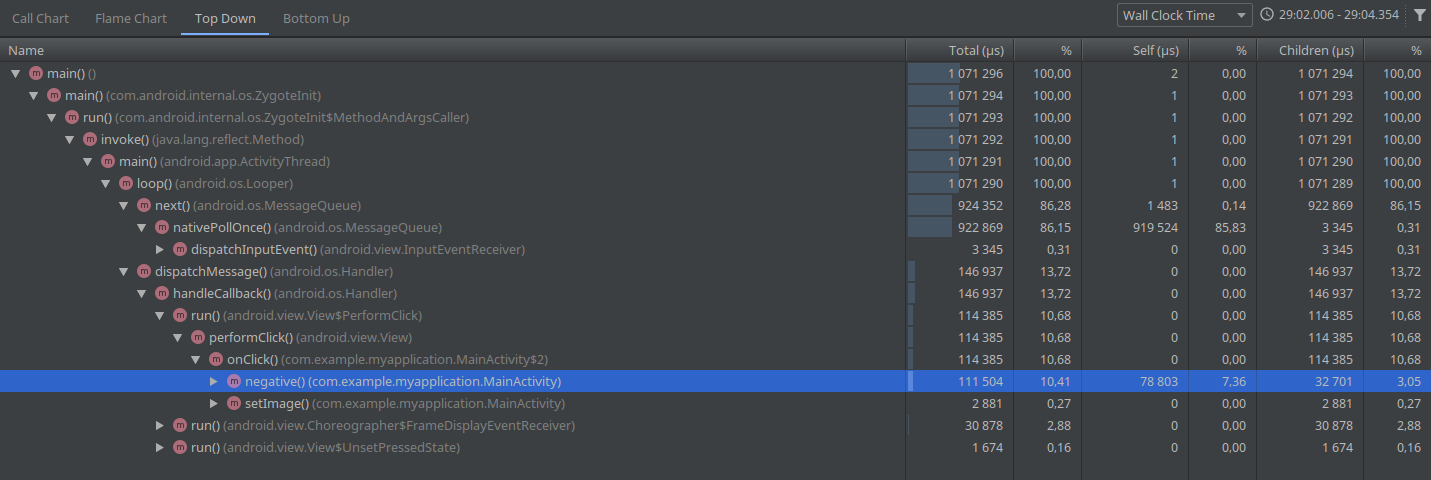
\includegraphics[width=11cm]{../Image_temps/TempsNegative}

    Temps de traitement de la fonction negative()
\end{center}

\newpage
\section{Interface \underline{TD 3 Question 3.1}}
Pour l'interface, j'ai décidé d'avoir un menu défilant horizontal permettant d'avoir tout les boutons accessibles dans un espace reduit.
\bigbreak 

Pour les fonctions modifiant la saturation et la luminosité et pour la sélection de couleur, j'ai voulu
Je souhaiterais en finalité utiliser une "seekbar" afin d'avoir quelque chose de plus visuel pour l'utilisateur.
\bigbreak

Je me suis aussi rendue compte que mon application ne s’adaptait pas aux barres de navigation virtuelles (contrairement au Neffos qui possède des boutons physique). En effet, certains boutons étaient cachés par la barre. 
J'ai donc résolu ce problème en modifiant la visibilité de l'interface utilisateur au lancement de l'application. Mais si on verrouille l'application et qu'on retourne dessus, on peut voir que la barre fixe revient, ce sera donc un problème à régler.


\end{document}